\chapter{Appendix B --- Rainfall Response of \passage{Vrtnarija} (2010)}


Assessing the flood response of the cave is obviously extremely important
with respect to the safety of the expedition members and continued
cave exploration. This year we had several periods of extended, extremely
heavy rain, whilst people were underground and the nature of the pitches
was inspected.

As well as for reasons of safety, due the expected difficulty in acquiring
permission to internally dye trace streams, comparing flow volumes
is the best method we have of understanding the hydrological connections
within our cave.

\subsection{\passage{Vrtnarija} Main Pitch Series}

\subsection{\passage{Laurel} to \passage{Pico}}


\begin{marginfigure}
\checkoddpage \ifoddpage \forcerectofloat \else \forceversofloat \fi
\centering
 \frame{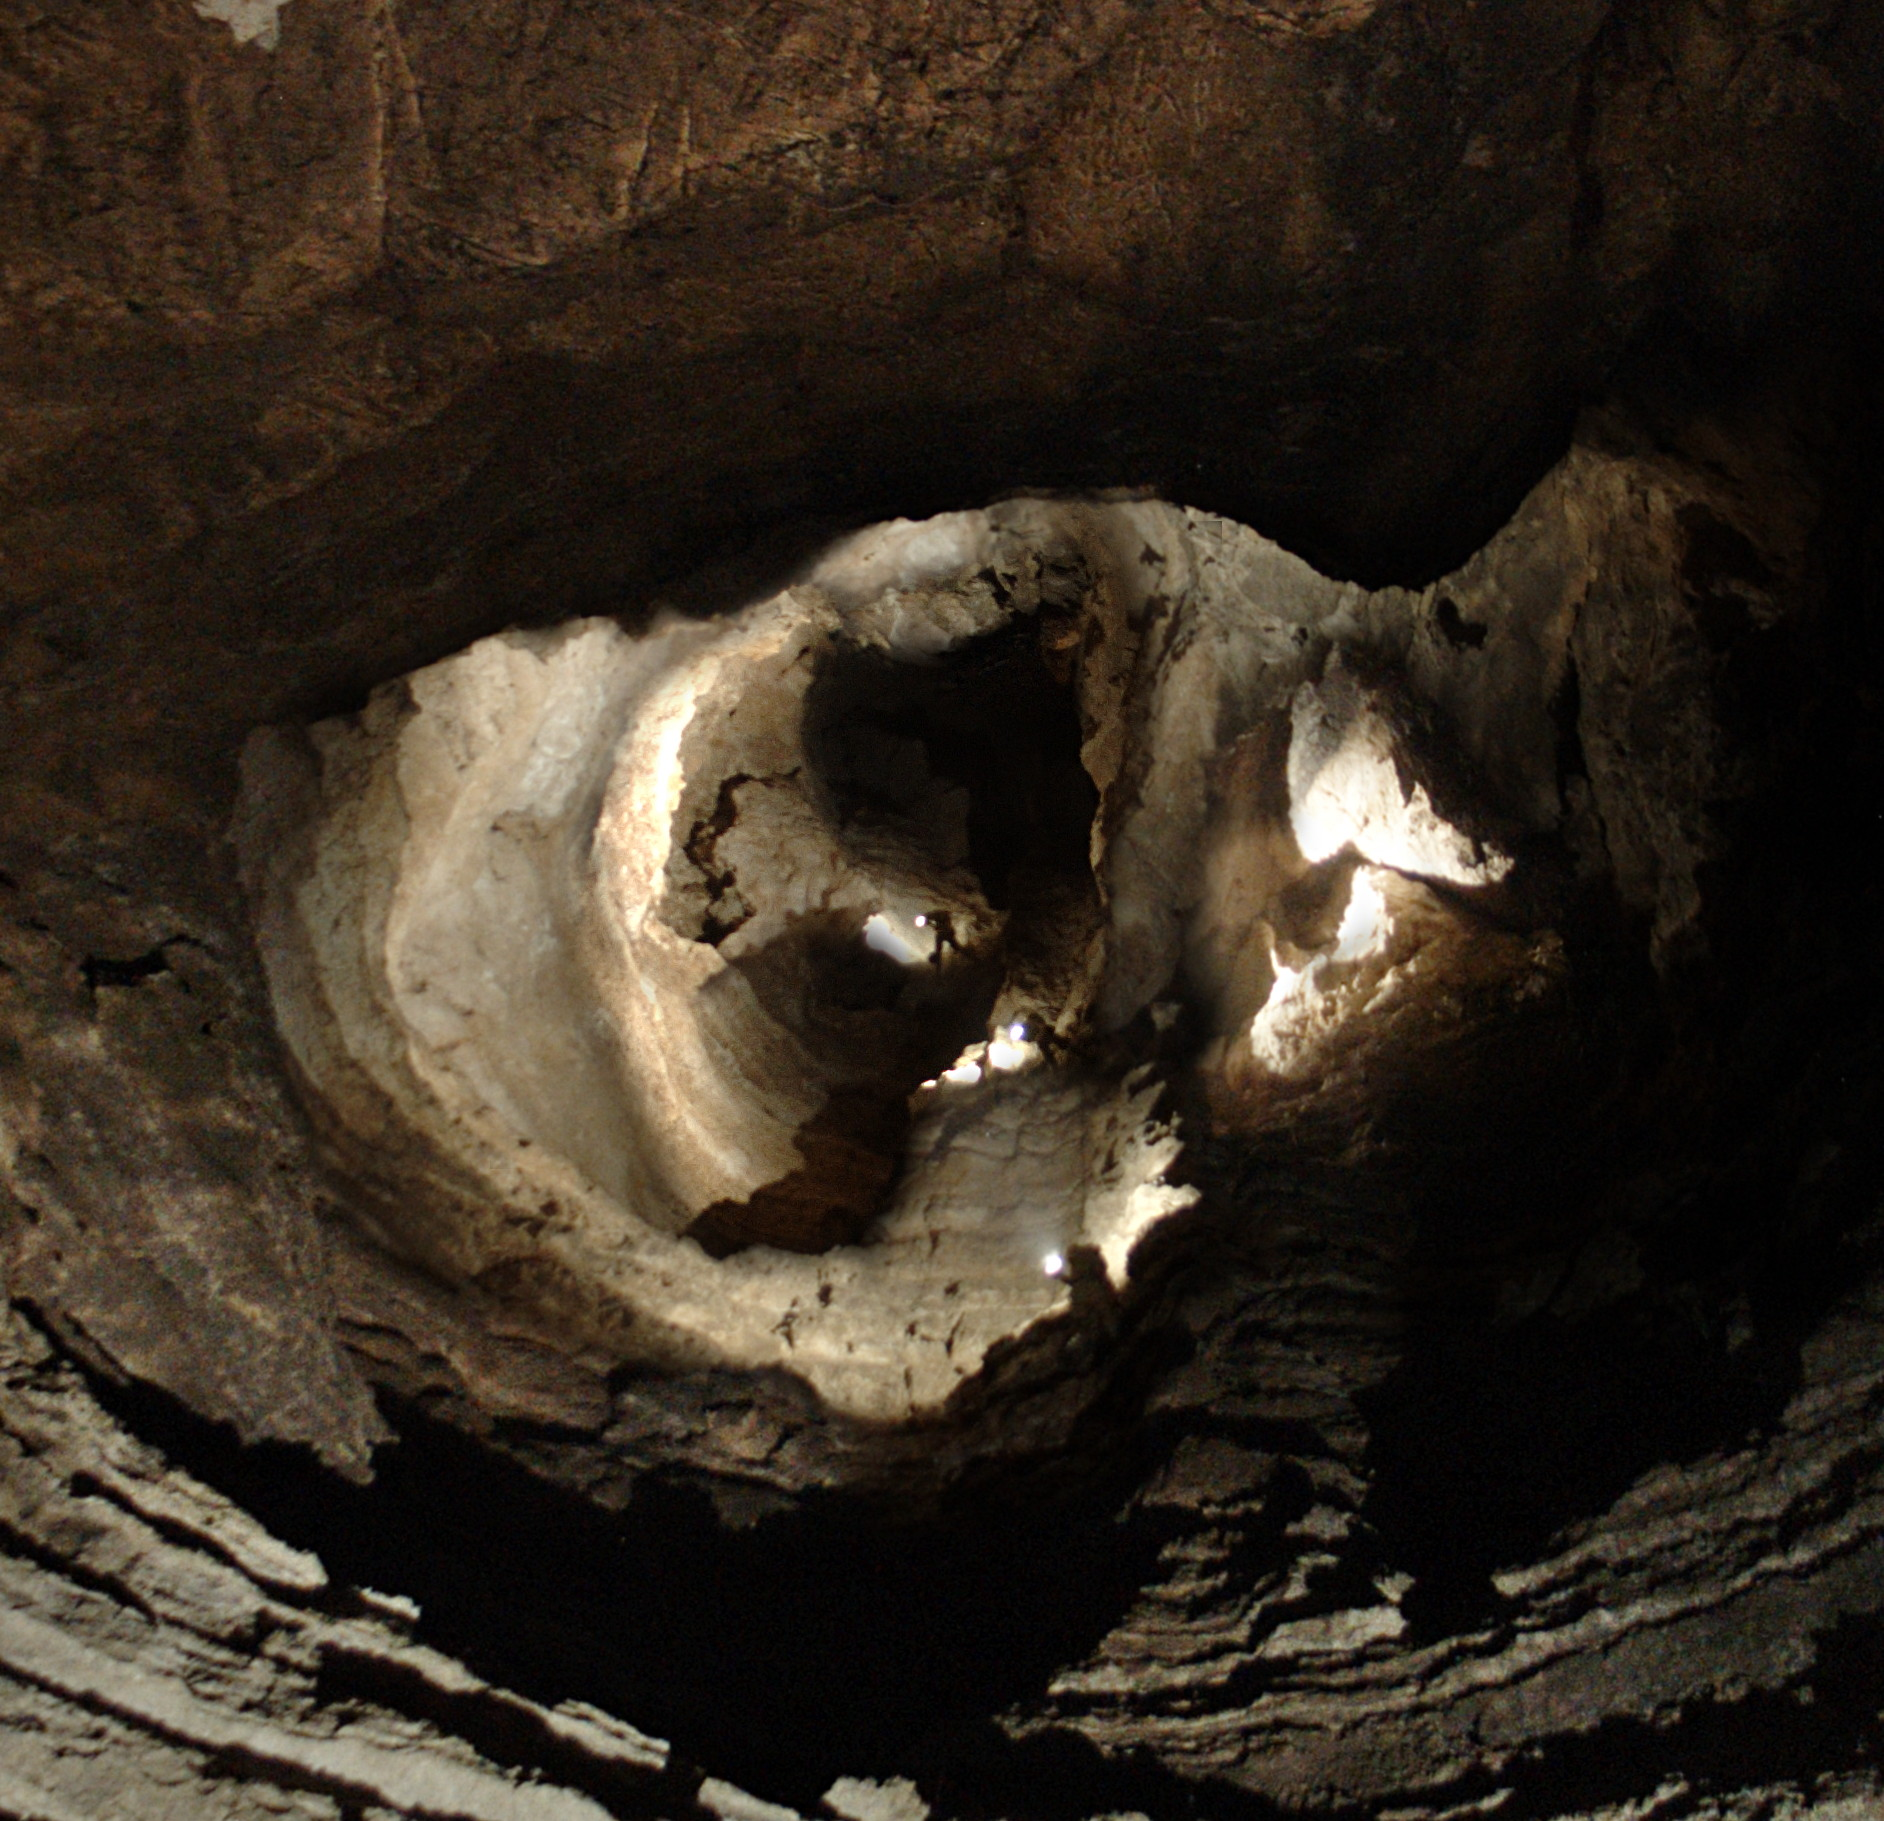
\includegraphics[width=\linewidth]{appendices/rainfall_response/2009-09-06-22.03.51 - Jarvist Frost - Canon Powershot G5 - Pico - composite square based--orig.jpg}} 
 \caption{\protect\passage{Pico} pitch. \pic{Jarvist Frost}}
 \label{pico square}
\end{marginfigure}


\passage{Laurel} gets very drippy during heavy rain (with a small stream entering through
an immature development part way down), but quickly clears after the end of the
storm. This water is followed to the top of \passage{Pico} (supplemented by a usually dry
inlet below \passage{I Scream}), but all pitches are rigged dry and fully passable. 
The water disappears below boulders at the top of \passage{Pico}, and is possibly
regained a short distance into \passage{Captain Kangaroo} where it forms the mostly
hidden stream in the immature rift which is followed to \passage{Bonus Chamber} where it
flows into a narrow rift (unpushed) below a boulder choke.

\subsection{\passage{Pico} to \passage{Pink}}

\passage{Pico} itself is rigged entirely dry, but an inlet splashes the far side of the
pitch. Again, this water is then followed down \passage{Terra}, \passage{Nova} and \passage{Swing}, but these
are also rigged dry. The water flows into a pool in \passage{The Officer's Club}, whereas
the main route follows a higher abandoned level. \passage{Tessellator} and the first hang
of \passage{Space Odyssey} are entirely dry, a considerable volume of water enters on the
bottom hang of \passage{Space Odyssey}. The rigging is entirely clear of the
water. This water then disappears down a hole down 'the back of' \passage{Concorde}.

\begin{marginfigure}
\checkoddpage \ifoddpage \forcerectofloat \else \forceversofloat \fi
\centering
 \frame{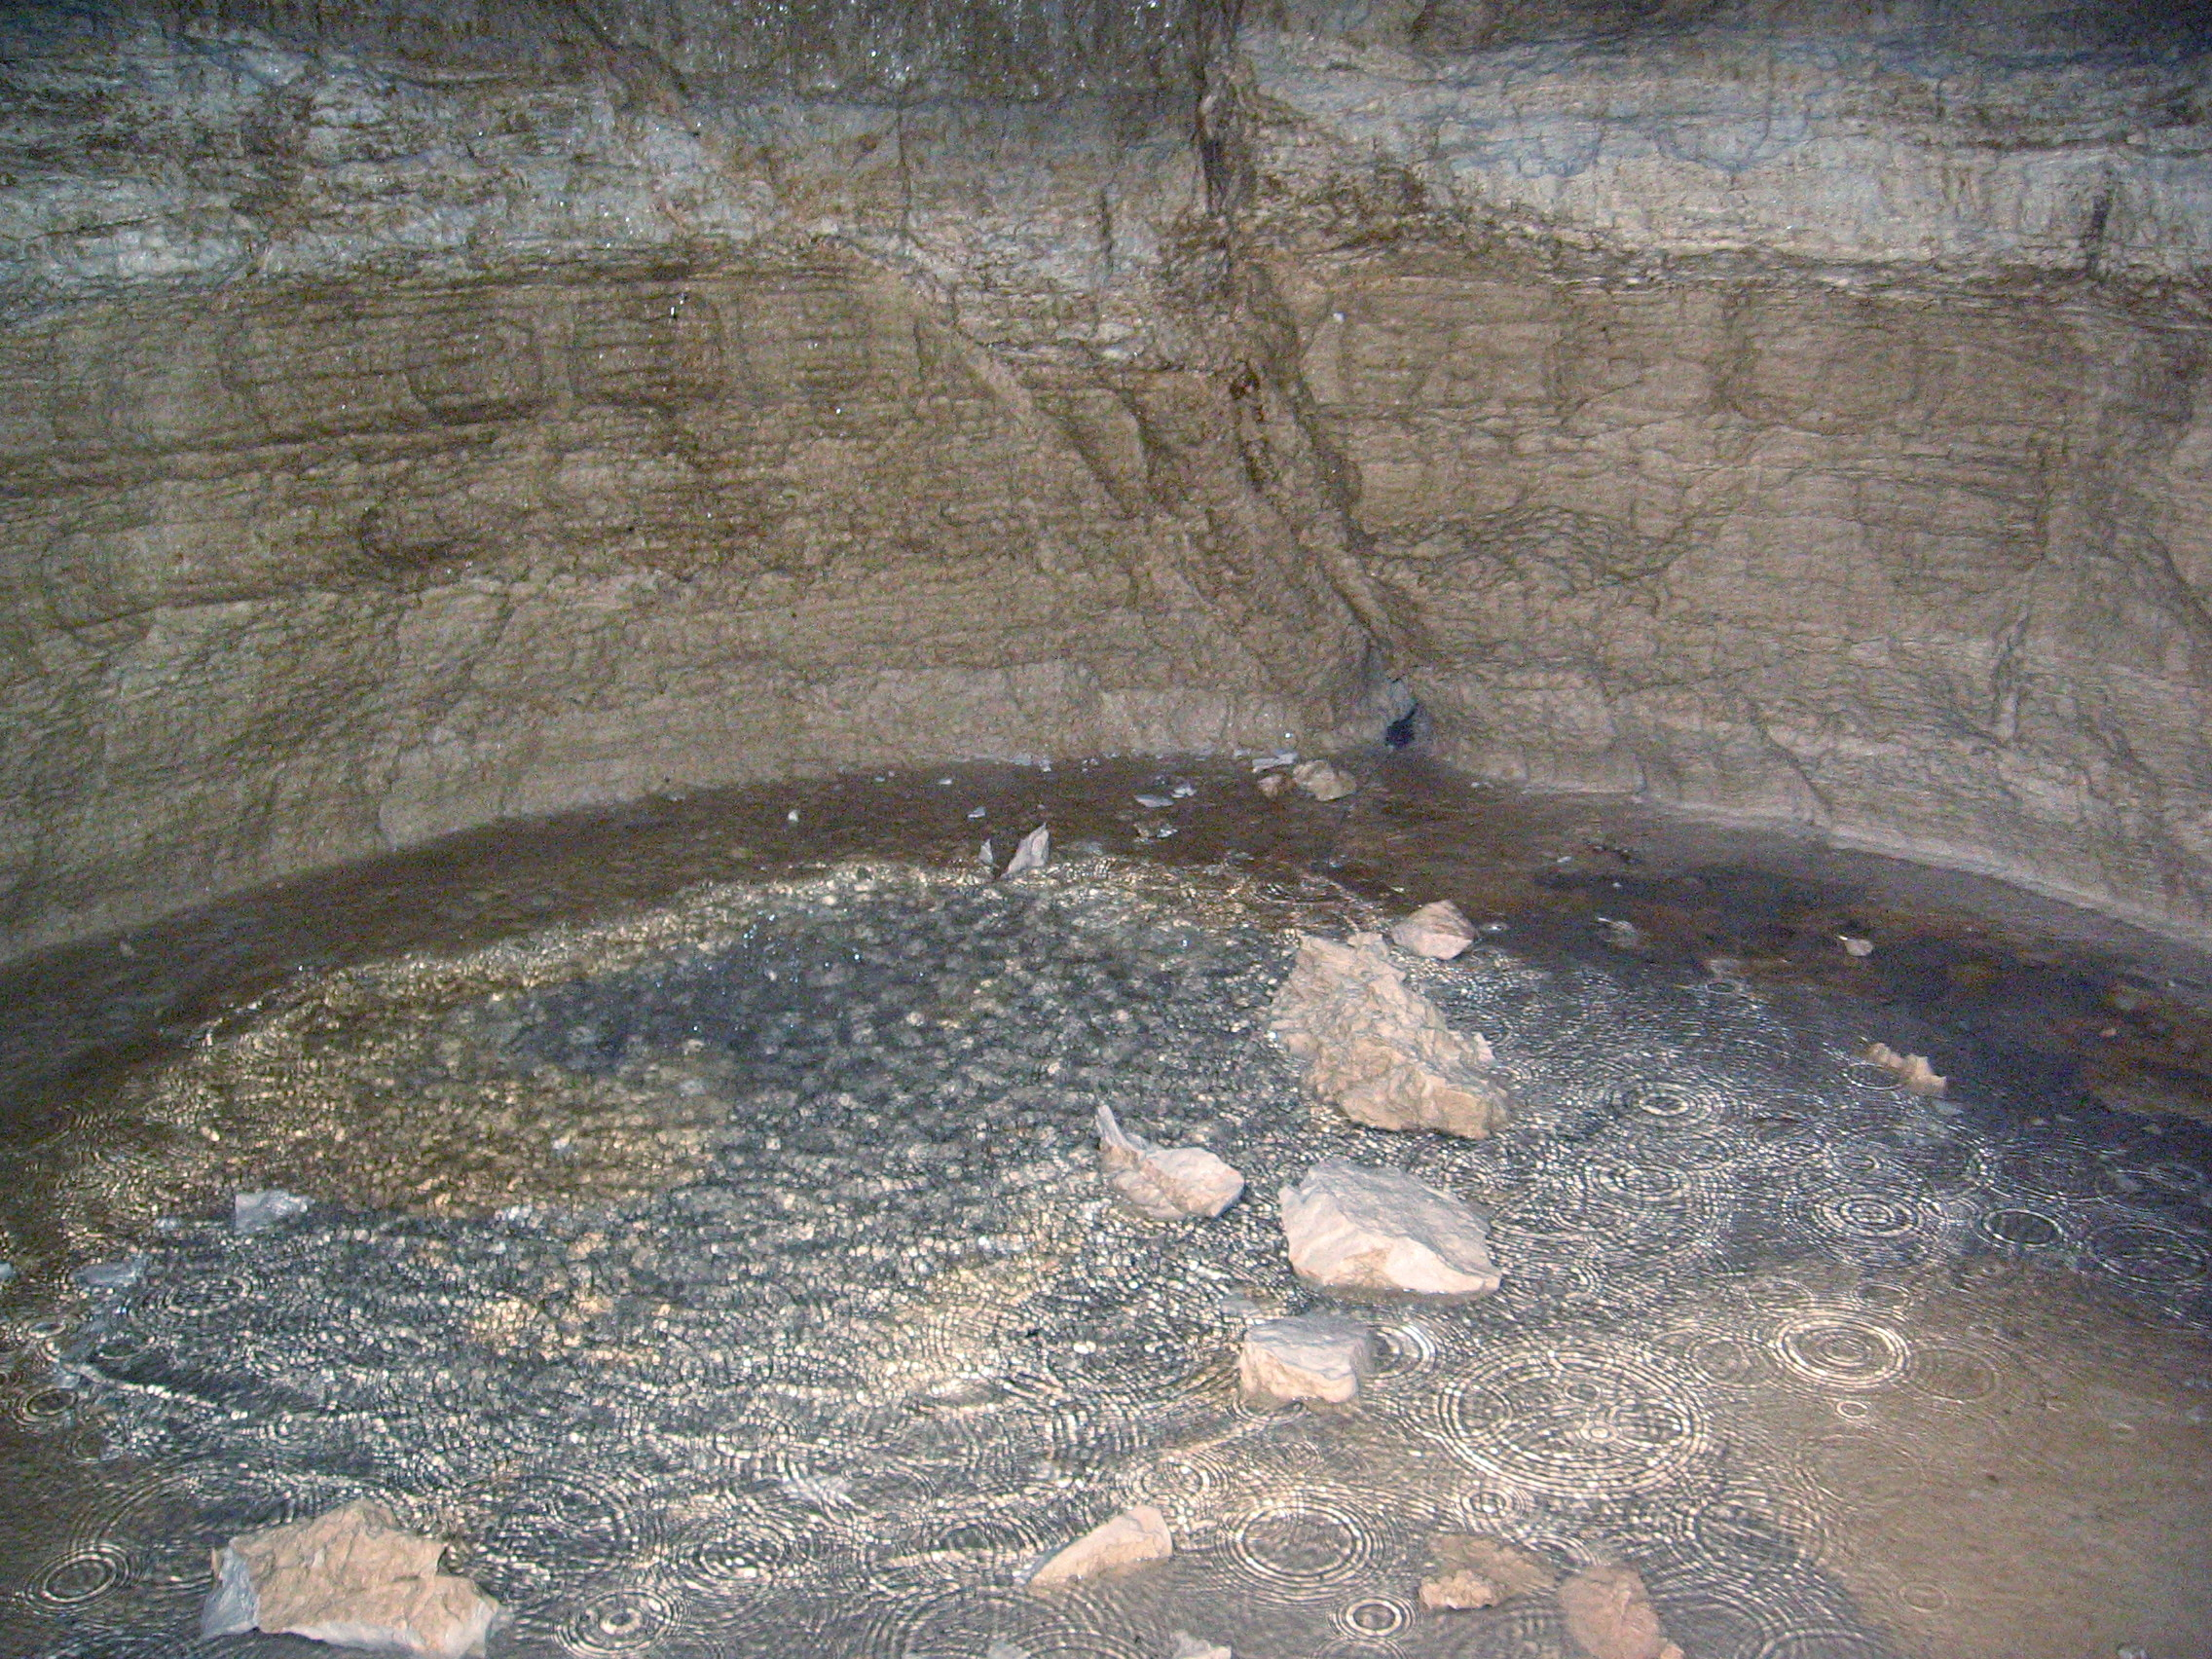
\includegraphics[width=\linewidth]{appendices/rainfall_response/2009-08-16-00.02.46 - Jana Carga - Canon Powershot A520 - Alchemy - drips--orig.jpg}} 
 \caption{The base of \protect\passage{Alchemy}. \pic{Jana Čarga}}
 \label{alchemy drips}
\end{marginfigure}

\passage{Concorde} itself is then mostly dry, with the last two rebelays being
slightly drippy. Strangely, the volume of drips does not seem to vary
much with rain on the surface. This small volume then flows 
down \passage{Alchemy}, \passage{Zlatorog} and \passage{Fistful of Tolars} (again, entirely separate
from the rope) and is believed to flow into the \passage{Banzai} streamway.

\subsection{\passage{Pink} to \passage{Zimmer}}

The first pitch in \passage{Pink} is dry under normal conditions --- with a considerable
volume of water entering out of a bedding plane in the rock and flowing over
the pitch about $\approx$ 5 m from the rigged location. However, heavy
rainfall can result in a sheet of water flowing closer to the final hang, and
even reaching it. 

The volume present on the first pitch in \passage{Pink} seems comparable to the amount
present on \passage{Space Odyssey} and it is thus hypothesised that the streams are the
same (i.e. there is a wet parallel pitch series). This water then disappears
(into an unpushed streamway, possibly joining into \passage{Banzai}). The rest of the
\passage{Pink} series is dry.

The lower hang in \passage{Skynet} takes a small stream during continual rain. The
bottom hang of \passage{Zimmer} and the rebelay is extremely wet during heavy rain
--- the lower half of the chamber is filled with heavy
flying spray. The water from \passage{Skynet} enters through a cut-back slot and bounces
off a series of ledges arriving at the floor in a chaotic mess. 
There is an additional, larger, volume of water that enters on the far side of
the \passage{Zimmer} pitch. The region of \passage{Zimmer} pitch between the \passage{Leopard} window and \passage{Korita}
remains dry, and this may offer an alternative, dry, SRT route. 

\begin{marginfigure}
\checkoddpage \ifoddpage \forcerectofloat \else \forceversofloat \fi
\centering
 \frame{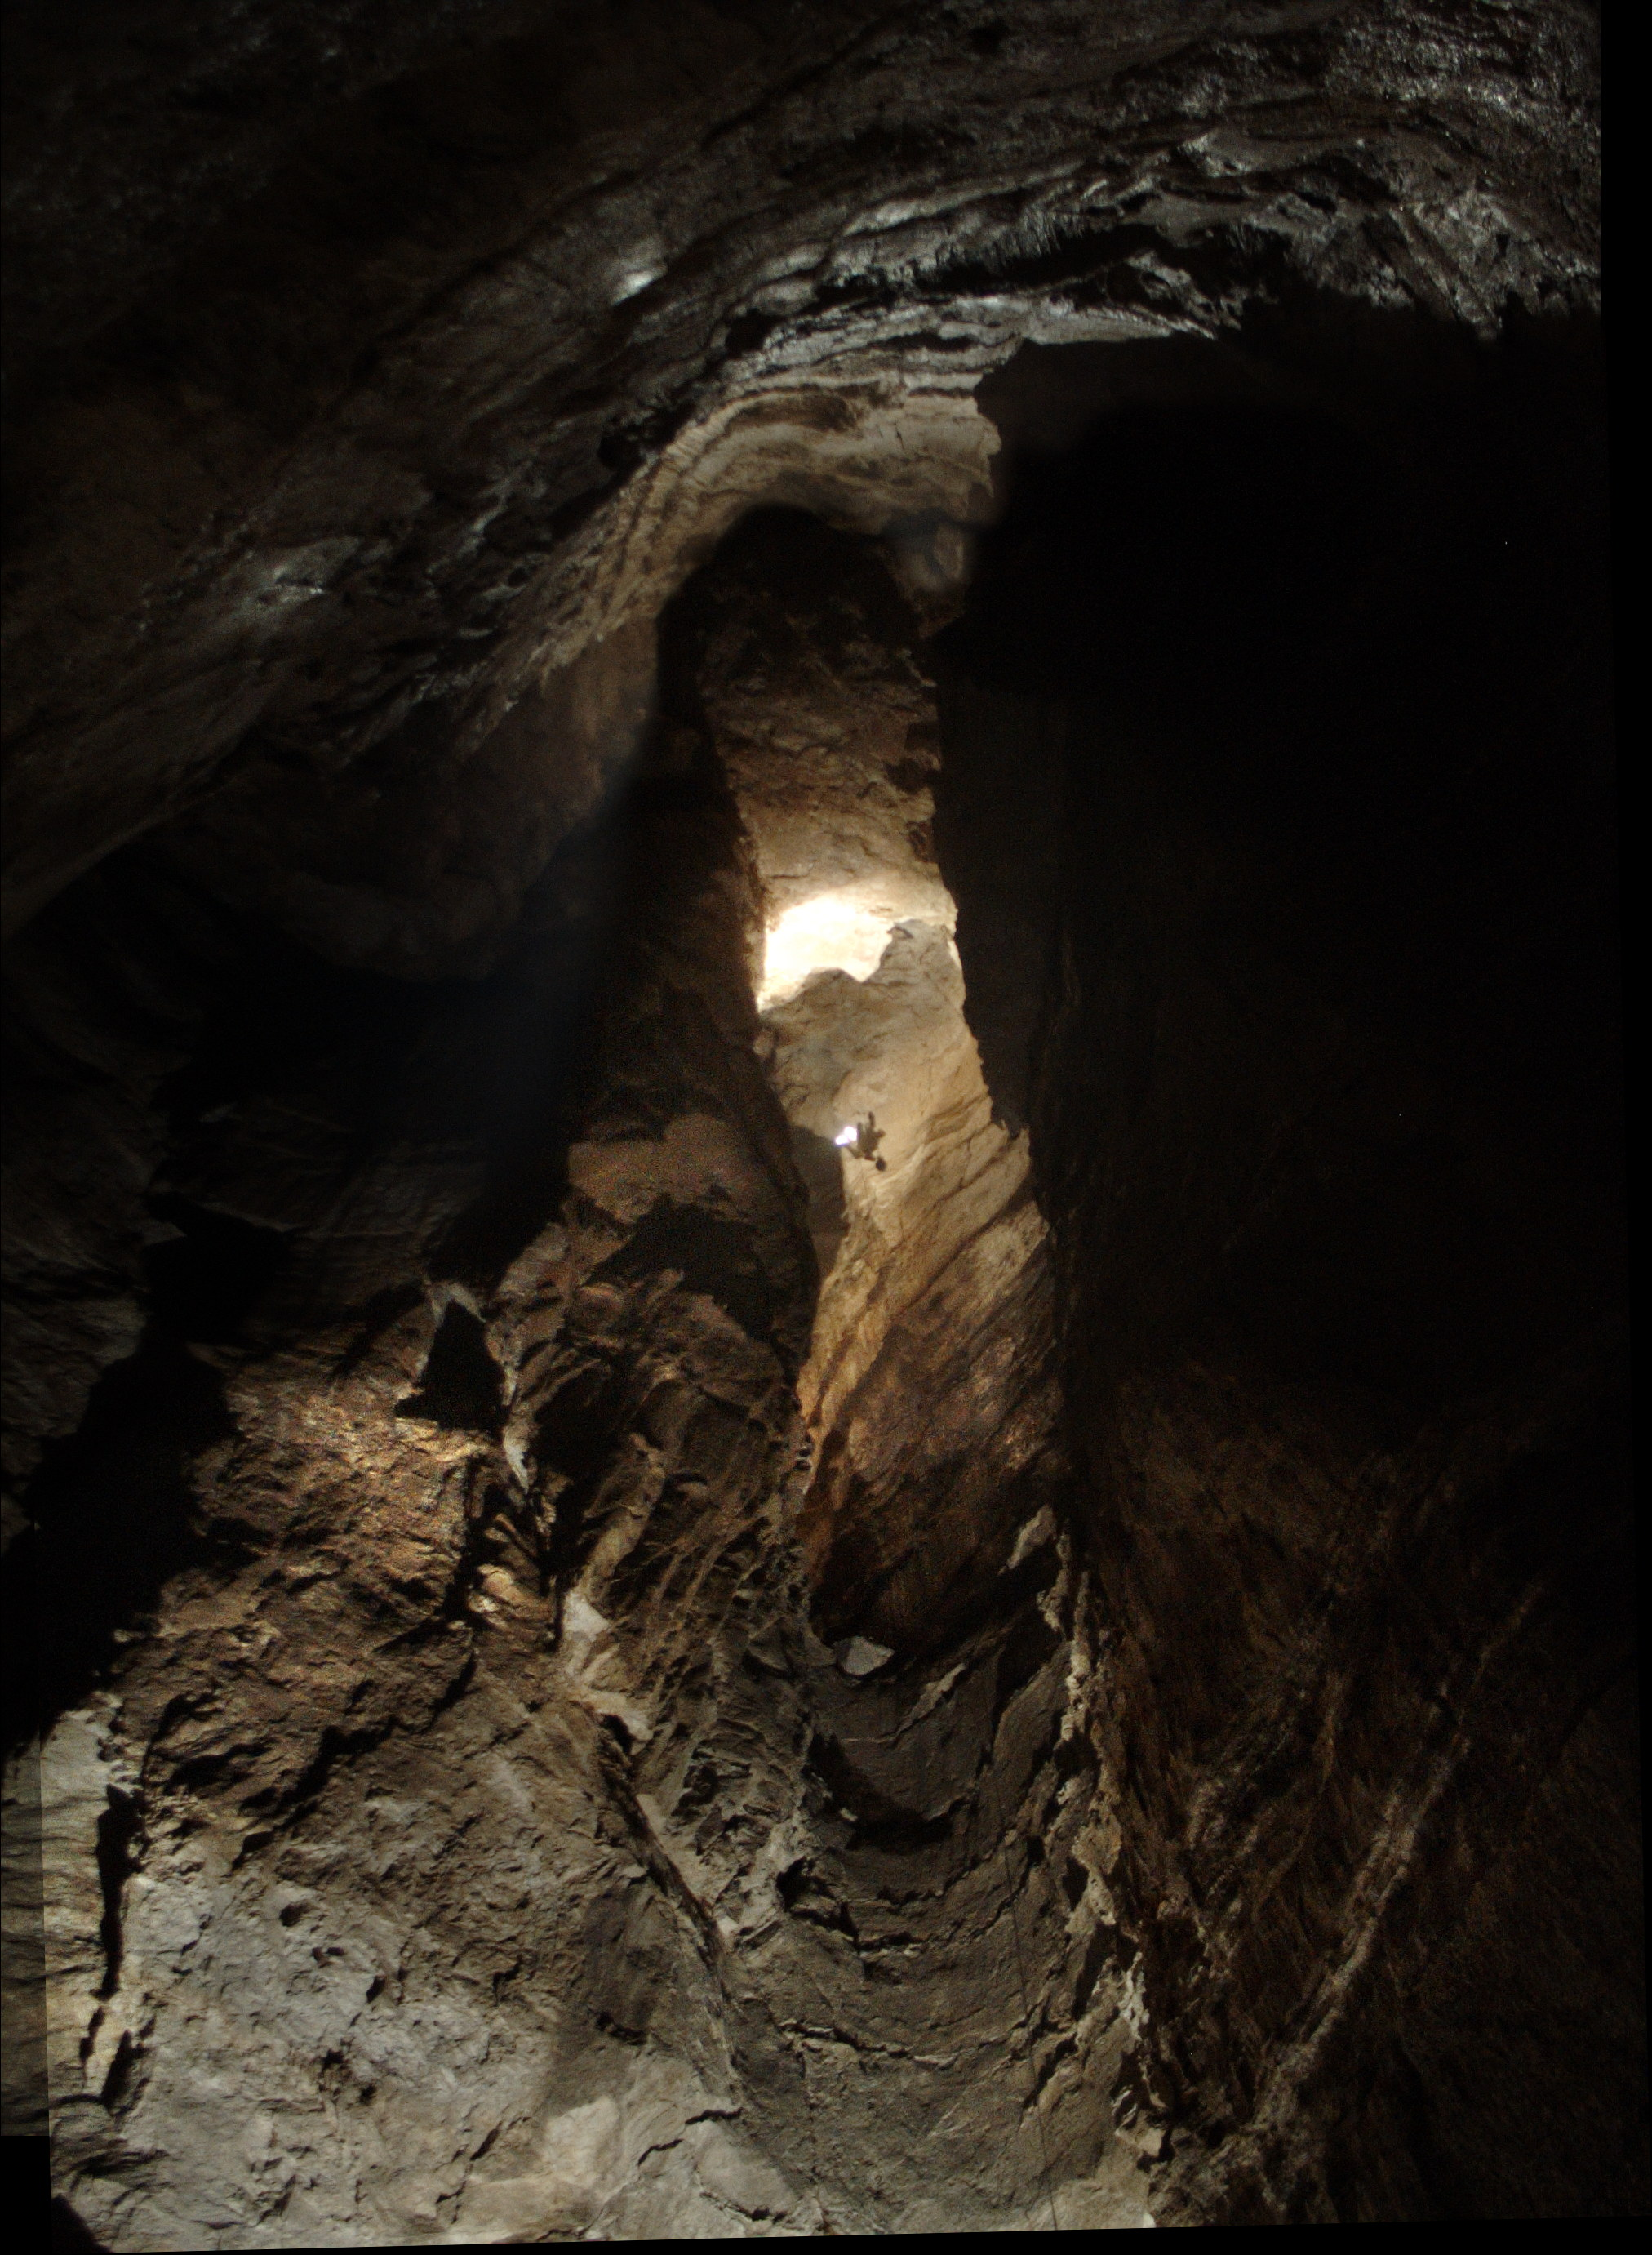
\includegraphics[width=\linewidth]{appendices/rainfall_response/2009-08-16-14.44.14 - Jarvist Frost - Canon Powershot G5 - zimmer composite--orig.jpg}} 
 \caption{Looking up \protect\passage{Zimmer}. \pic{Jarvist Frost}}
 \label{zimmer composite}
\end{marginfigure}

We currently believe that the water on \passage{Zimmer} collects under the boulders, then
flows down \passage{Korita} and is followed all the way to \passage{Crack in Time}.

Interestingly, during heavy rain, the draught changes direction in
\passage{Friendship Gallery}. The usual direction is from \passage{Zimmer} into \passage{Friendship Gallery}.
This reverses and strengthens during storms on the surface.

The first pitch in \passage{Pink} and \passage{Zimmer} are rerig targets for 2011. Once
rerigged, \passage{Vrtnarija} should be fully passable to and from camp, if not pleasant,
in all water conditions.

\subsection{\passage{Leopard}}

The main horizontal passages are entirely dry - except for passing
the first streamway, where a rebelay on the traverse was found to
be under the main flow during a flood pulse! Rerigging with a short
pitch down to the boulder choke pit and another at the far side has
been hypothesised for 2011. All of \passage{Wonderland} and the \passage{Palace of King
minos} is dry. The vertical leads following streamways, naturally,
are not.


\subsection{\passage{Korita}}

During a flood pulse all the pitches were found to be passable, except
for the top hang of \passage{Black Knight} pitch, where the deviation was found
to be submarine. A considerable flow existed in the tight rifts and
so drenched feet were a constant risk.


\subsection{\passage{Republica}}

The region was found to be fairly damp - with falling water in heavy conditions
soaking a rebelay. 

\passage{Big Rock} is drippy, but entirely passable.

\name{Jarvist Frost}